%
% !TEX root = ../../buch.tex
% !TEX encoding = UTF-8
%
%
% teil3.tex -- Hybrid mit Newton-Verfahren und Einordnung
%
\section{Hybrid mit dem Newton-Verfahren und Einordnung%
\label{weyl:section:hybrid}}
\kopfrechts{Hybrid mit Newton-Verfahren}
Der Quadtree-Algorithmus ist global und zuverlässig, aber langsam. Pro Iteration
verdoppelt sich die Genauigkeit lediglich um ein Bit.
Das Newton-Verfahren ist hingegen lokal sehr schnell. In der Nähe einer einfachen
Nullstelle verdoppelt sich die Anzahl korrekter Stellen pro Schritt. Das Verfahren ist aber empfindlich
gegenüber dem Startwert und kann bei ungenauem Startwert versagen.
Es liegt nahe, beide Verfahren zu kombinieren und so von beiden Stärken zu profitieren.

\subsection{Wann der Quadtree an Newton übergibt%
\label{weyl:subsection:uebergabe}}
Sobald ein Quadtree-Quadrat $D_i$ mit $N(D_i) = 1$ klein genug ist, liegt seine
Mitte $\hat z$ in unmittelbarer Nähe der einzigen Nullstelle in diesem Quadrat.
``Klein genug'' bedeutet dabei, dass $\hat z$ im Einzugsgebiet des Newton-Verfahrens
für genau diese Nullstelle liegt. Sind die Nullstellen ausreichend weit voneinander
getrennt, genügt dafür schon eine sehr moderate Genauigkeit des Quadtree.
Ab diesem Punkt schalten wir um auf die Newton-Iteration
\begin{equation}
z_{k+1}
=
z_k
-
\frac{f(z_k)}{f'(z_k)}
,
\quad
z_0
=
\hat z
,
\label{weyl:eq:newton}
\end{equation}
die quadratisch gegen die Nullstelle konvergiert.
Aus dem Startwert $\hat z$, der bereits einige Stellen Genauigkeit hat, wird so in
wenigen Schritten Maschinenpräzision erreicht.
Ein praktischer Test, ob das Quadrat klein genug war, besteht darin, die ersten
Newton-Iterierten zu beobachten.
Bleiben sie im aktiven Quadrat $D_i$, spricht das dafür, dass der Startwert im
richtigen Einzugsgebiet liegt.
Verlässt die Folge das Quadrat oder springt sie stark, verfeinert man $D_i$ weiter
und versucht die Übergabe erst mit einem kleineren Quadrat erneut.

%
% fig/hybrid.tex -- Übergang Quadtree -> Newton
%
\begin{figure}
\centering
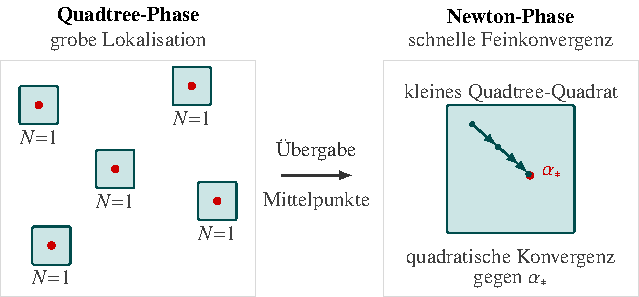
\includegraphics{papers/weyl/images/hybrid.pdf}
\caption{Hybrid-Strategie: links liefert der Quadtree-Algorithmus für jede Nullstelle
ein kleines Quadrat mit $N(D_i) = 1$, das nur noch eine einzige Nullstelle enthält.
Die Mittelpunkte dieser Quadrate dienen als Startwerte $z_0$ für das
Newton-Verfahren (rechts), das in wenigen Schritten quadratisch gegen die wahre
Nullstelle $\alpha_*$ konvergiert. So vereinen sich die globale Zuverlässigkeit des
Quadtree und die lokale Geschwindigkeit von Newton.
\label{weyl:fig:hybrid}}
\end{figure}


Abbildung~\ref{weyl:fig:hybrid} skizziert das Zusammenspiel:
Der Quadtree übernimmt die globale Lokalisation und garantiert, dass jede Nullstelle
gefunden wird. Das Newton-Verfahren übernimmt die schnelle Feinkonvergenz auf den
letzten Metern.
Natürlich kann man alle Nullstellen auch anders suchen. Hat man eine Nullstelle
$\alpha$ numerisch gefunden, kann man den Faktor $(z-\alpha)$ abspalten und im
deflationierten Polynom weiterrechnen. Der Nachteil ist, dass der numerische Fehler
von $\alpha$ in die Koeffizienten des neuen Polynoms eingeht und dadurch die
Genauigkeit der später gefundenen Nullstellen beeinträchtigen kann.
Beim Weyl-Algorithmus tritt dieses Problem nicht auf, weil die Nullstellen in
verschiedenen Quadraten \emph{unabhängig} voneinander lokalisiert werden. Sobald der
Baum mehrere aktive Quadrate enthält, können diese Teilprobleme sogar parallel
bearbeitet werden.

\subsection{Stärken und Schwächen%
\label{weyl:subsection:einordnung}}
Welche Eigenschaften zeichnen das Verfahren aus?
Wir fassen zusammen, was wir gewonnen haben und was es ``kostet''.

\subsubsection*{Stärken}
Der Quadtree-Algorithmus ist \emph{global zuverlässig}.
Wenn das Startquadrat alle Nullstellen umschliesst, garantiert er, dass keine Nullstelle
übersehen wird, was durch die Probe \eqref{weyl:eq:probe} auf jeder Stufe geprüft wird.
Er erfordert, anders als beim reinen Newton-Verfahren, \emph{keine Startwerte}. 
So muss man nicht raten, wo die Nullstellen liegen.
Die Anzahl der Nullstellen in einem Gebiet ist von Anfang an bekannt, da sie das
\emph{Argumentprinzip} als Nebenprodukt liefert.
Mehrfache Nullstellen werden zwanglos behandelt, indem das Verfahren sie
automatisch erkennt durch $N(D_i) \geq 2$.

\subsubsection*{Schwächen}
Die Konvergenz ist nur \emph{linear} (jede Iteration halbiert den Fehler), nicht
quadratisch wie bei Newton.
Alleine angewendet wäre Weyls Algorithmus zu langsam für hohe Genauigkeitsanforderungen.
Erst die Kombination mit Newton macht ihn praxistauglich.
Jede Iteration kostet zudem vier Wegintegrale pro Elternquadrat, welche nicht ganz
billig sind, vor allem wenn das Polynom hohen Grad hat oder das Gebiet viele Quadrate
enthält.

\subsubsection*{Komplexität}
Bei einer geforderten Genauigkeit $\varepsilon$ braucht der Quadtree
$O(\log(r/\varepsilon))$ Verfeinerungsstufen.
Pro Stufe sind höchstens $O(n)$ Quadrate aktiv (da nur Quadrate mit
Nullstellen überleben) und in jedem Quadrat kostet die numerische Auswertung des
Wegintegrals $O(n)$ Funktionsauswertungen.
Insgesamt landet man so bei einer Komplexität in der Grössenordnung
$O\bigl(n^2 \log(r/\varepsilon)\bigr)$ Polynomauswertungen für die
Quadtree-Phase. Hinzu kommen wenige Newton-Schritte pro Nullstelle für die
Feinkonvergenz.
Detaillierte Schranken und Varianten sind in \cite{weyl:pan1998} diskutiert.

\subsection{Historische und praktische Einordnung%
\label{weyl:subsection:historisch}}
Hermann Weyl hat den Algorithmus 1924 in \cite{weyl:weyl1924} vorgeschlagen, lange vor
dem Aufkommen von Computern.
Im Kontext seiner Zeit war das Verfahren vor allem theoretisch bemerkenswert.
Es liefert einen \emph{konstruktiven Beweis} des Fundamentalsatzes der Algebra, der die
Nullstellen tatsächlich lokalisiert.
\index{konstruktiver Beweis}%
Mit dem Aufkommen numerischer Rechner wurde der Algorithmus in mehreren Arbeiten
weiterentwickelt, etwa um effiziente Integrationsmethoden, robustere Abbruchkriterien
und bessere Komplexitätsschranken
\cite{weyl:pan1998}.

In heutigen Standard-Solvern für komplexe Polynomnullstellen werden zwar meist
matrixbasierte Verfahren wie die Eigenwertberechnung der Begleitmatrix mit dem
\index{Eigenwertberechnung}%
$\mathit{QR}$-Algorithmus eingesetzt. Das Grundprinzip von Weyls Algorithmus --- Gebiete
\index{QR-Algorithmus}%
unterteilen und mit dem Argumentprinzip auf Nullstellen testen --- lebt jedoch in
modernen \emph{Inclusion-Test}-Methoden weiter, etwa in den Arbeiten zu
zuverlässigen Polynomwurzel-Solvern.
\index{Inclusion-Test}%
Weyls Quadtree ist damit nicht nur historisch interessant, sondern ein Vorbild für
heutige robuste Solver, die Garantien statt nur Näherungen liefern wollen.

\subsection{Fazit%
\label{weyl:subsection:fazit}}
Weyls Quadtree-Algorithmus ist ein elegantes Beispiel dafür, wie ein klassisches
Resultat der komplexen Analysis (das Argumentprinzip) als Konsequenz des Cauchy-Integralsatzes
in ein konstruktives, geometrisches Verfahren übersetzt werden kann.
Die zentrale Idee, durch Faktorisieren des Polynoms die Nullstellen in Polstellen der
logarithmischen Ableitung $f'/f$ zu verwandeln und sie dann durch ein Wegintegral
zählen zu lassen, ist von bestechender Einfachheit.
Sie macht das Bisektionsprinzip in der komplexen Ebene nutzbar und liefert einen
zuverlässigen Lokalisator, den man dann an das schnelle, aber wählerische
Newton-Verfahren übergibt.
So ergänzen sich Geometrie und Numerik zu einem Verfahren, das robust ist, sich seines
Fortschritts bewusst ist und letztlich keine Nullstelle übersieht.
